\chapter{Classification \label{chapter:classification}}

Classification is a form of \textbf{supervised learning} in which our goal is to learn a mapping between some features, $x$, and an output, $y$. The general setup for supervised learning looks like this:
\begin{center}
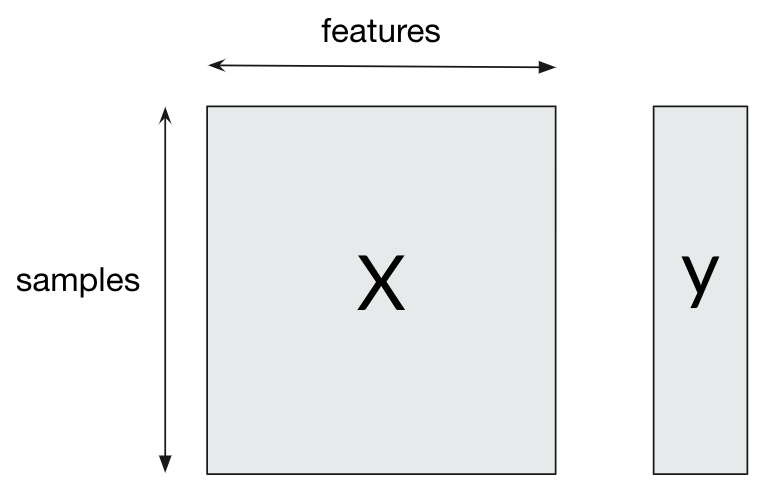
\includegraphics[width=0.7\textwidth]{img/supervised-learning.png}
\end{center}

In classification, the output, $y$, is a category. In \textbf{binary classification} (by far the most common), there are only two categories: yes or no, usually represented as ``0'' (no) or ``1'' (yes). In \textbf{multi-class classification}, there are more than two categories.

To learn an appropriate mapping, we feed \textbf{training data} to a \textbf{learning algorithm}. Different algorithms learn different types of mappings.

\section{Definitions}

\begin{itemize}
\item \textbf{Training data:} The data used, along with an appropriate learning algorithm, to create the mapping between input and output. It is composed of \textbf{samples}, each consisting of one or more input features and a single output.
\item \textbf{Test data:} An independent dataset, not used in model training, on which the performance of a trained supervised learning model is evaluated. 
\item \textbf{Feature:} Also known as a \textbf{predictor}, or \textbf{covariate}, one of the inputs to a supervised learning algorithm.
\item \textbf{Output:} Also known as the \textbf{outcome}, or \textbf{label}, the thing you are trying to predict.
\item \textbf{Feature space:} Envisioning each feature as having its own axis that is orthogonal to all of the other features' axes, the multidimensional space spanned by those axes (or rather: unit vectors in the directions of those axes)
\item \textbf{Extrapolation:} Making predictions outside the region of the feature space occupied by the training data. This will often lead to errors. 
\end{itemize}

%%%%%%%%%%%%%%%%%%%%%%%%%%%%%%%%%%%%%%%%%%%%%%%%%%%%%%%%%%%%%%%%%%%%%%%%%%%%%%%%%%%%%%

\section{Visualizing the Classification Problem \label{section:visualizingclass}}

Imagine we want to predict whether a patient will be readmitted to the emergency room (ER) within $30$~days of discharge from the hospital. We gather data on two predictors: a disease severity score ($x_1$), which characterizes the severity of the illness for which the patient was treated during his/her admission, and a social determinants score ($x_2$), which characterizes a patient's socioeconomic status. We gather data on $200$~distinct patients.

In the figure below, the color refers to whether a patient was admitted to the emergency room (ER) within 30 days of discharge (blue = ``no'', red = ``yes''). The location of each point is governed by the patient's disease severity score ($x_1$, horizontal axis) and social determinants score ($x_2$, vertical axis).

\begin{center}
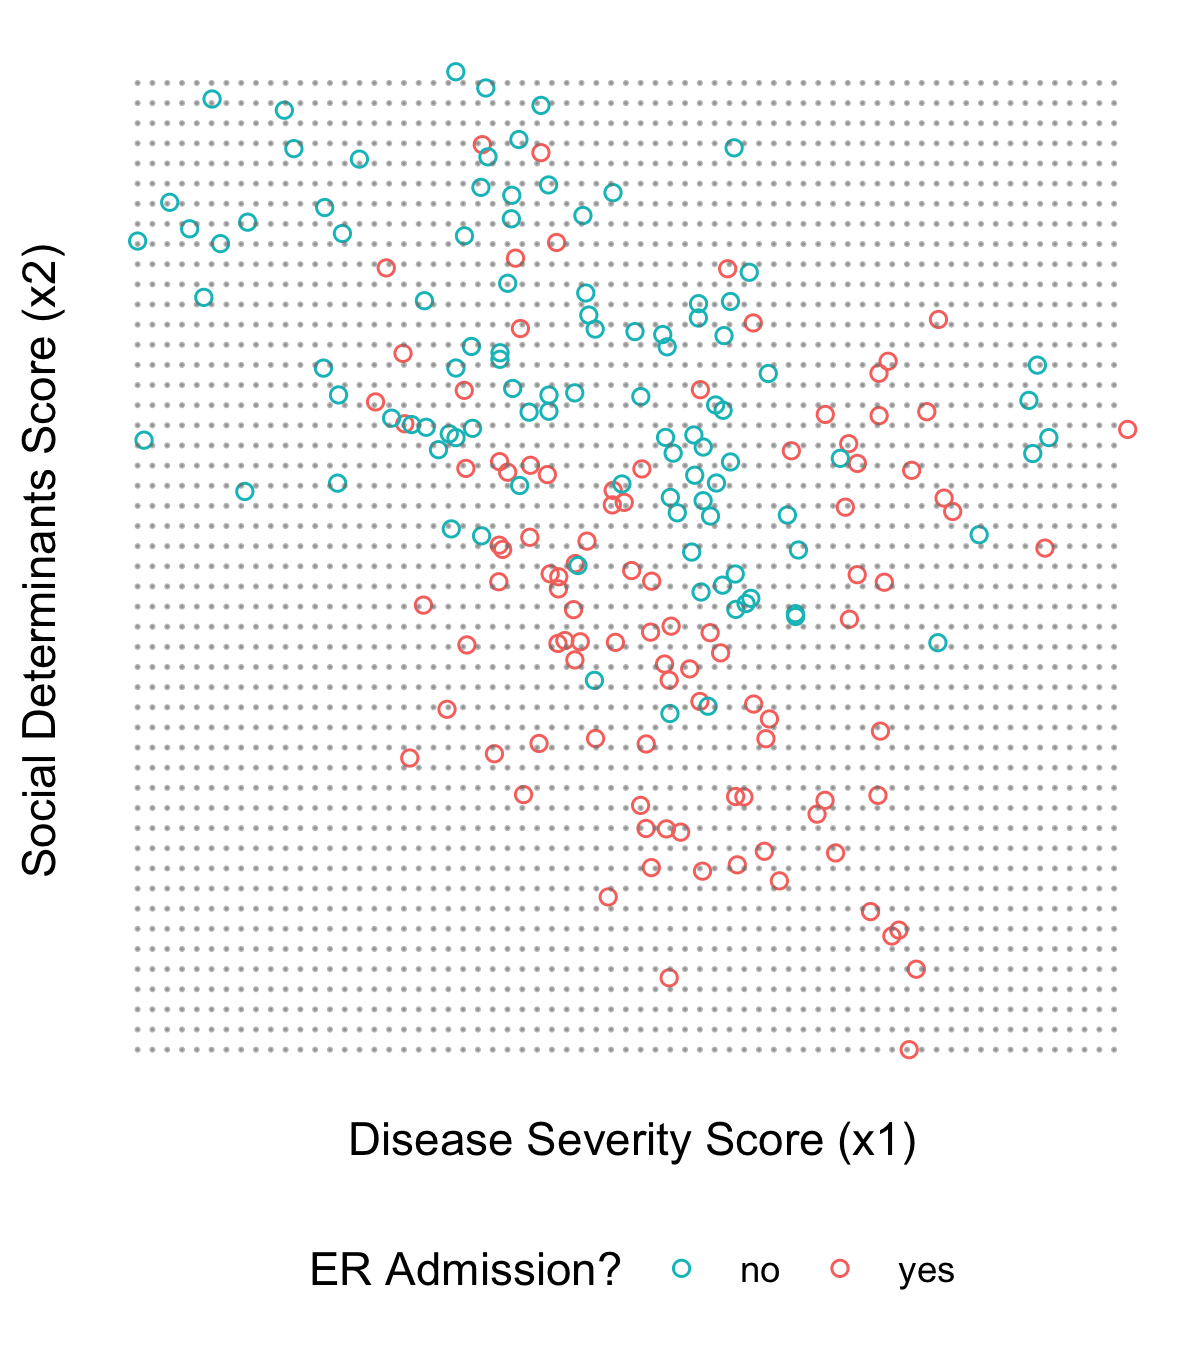
\includegraphics[width=0.7\textwidth]{img/esl-just-data.png}
\end{center}

Our goal in classification is to draw a \textbf{decision boundary}\index{decision boundary} through this space, on one side of which we will predict the patient to be readmitted, and on the other side of which we will predict the patient \emph{not} to be readmitted. The question in classification is: How do we draw a good boundary? How do we draw a boundary that will lead to accurate predictions on patients our model has never seen before?

%%%%%%%%%%%%%%%%%%%%%%%%%%%%%%%%%%%%%%%%%%%%%%%%%%%%%%%%%%%%%%%%%%%%%%%%%%%%%%%%%%%%%%

\section{Three Classification Algorithms}

\subsection{Logistic Regression}

The simplest decision boundary is, arguably, a line. The logistic regression\index{logistic regression} algorithm simply draws a line\footnote{In a higher-dimensional feature space, the decision boundary for logistic regression is a \textbf{hyperplane}.} through the feature space that divides the positive and negative training examples. 

\begin{center}
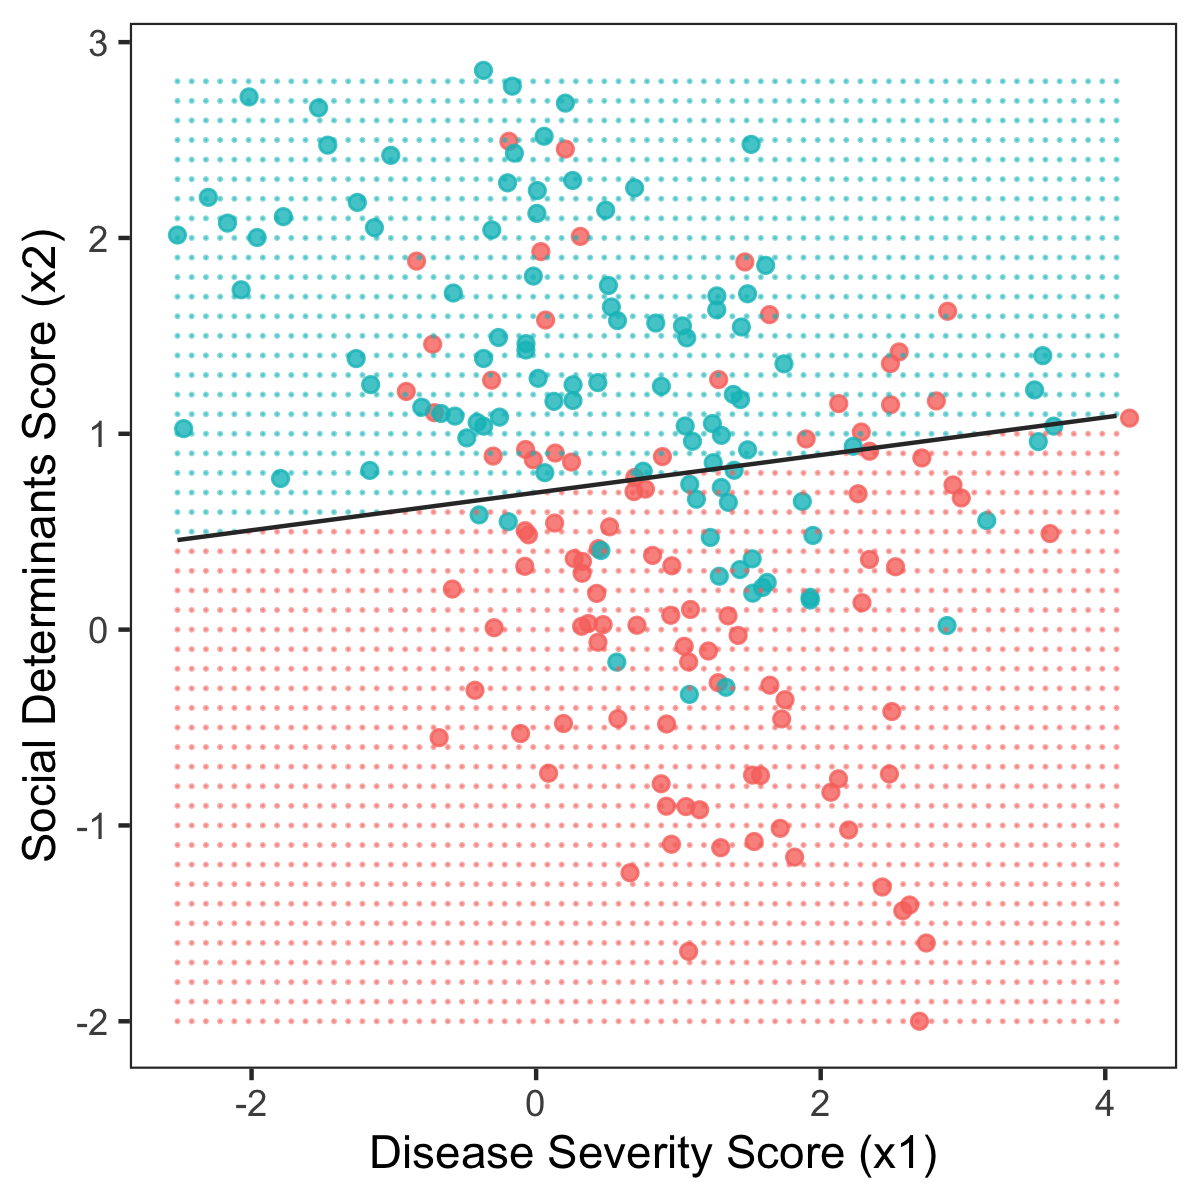
\includegraphics[width=0.7\textwidth]{img/esl-logistic.png}
\end{center}

\subsection{K Nearest Neighbors (KNN)}

Another approach is to make no assumptions about the shape of the decision boundary. To make a prediction about a new patient, we simply allow the $K$ nearest neighbors to vote. The parameter $K$ must be set independently and is called a \textbf{hyperparameter}. 

\noindent Here is the decision boundary for KNN with $K=15$:
\begin{center}
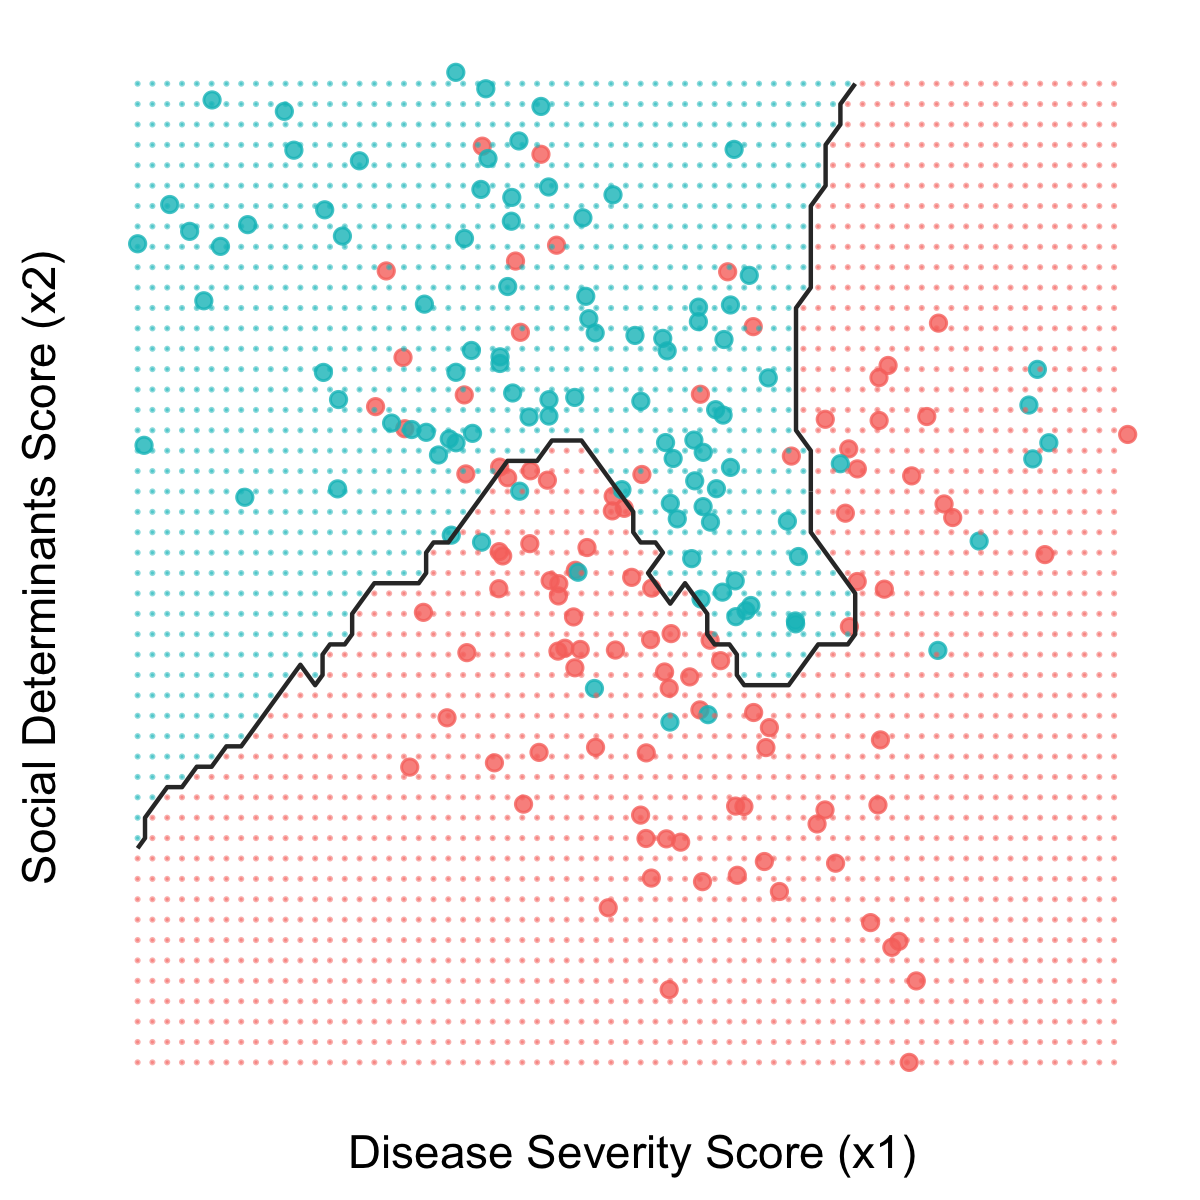
\includegraphics[width=0.7\textwidth]{img/esl-knn-15.png}
\end{center}

\subsection{Decision Tree}

Finally, we may choose to use our training data to build a decision tree\index{decision tree}, which will allow us to make predictions on new patients using a series of simple yes/no questions. There are different decision tree learning algorithms, but here is the tree produced by a famous one called CART:
\begin{center}
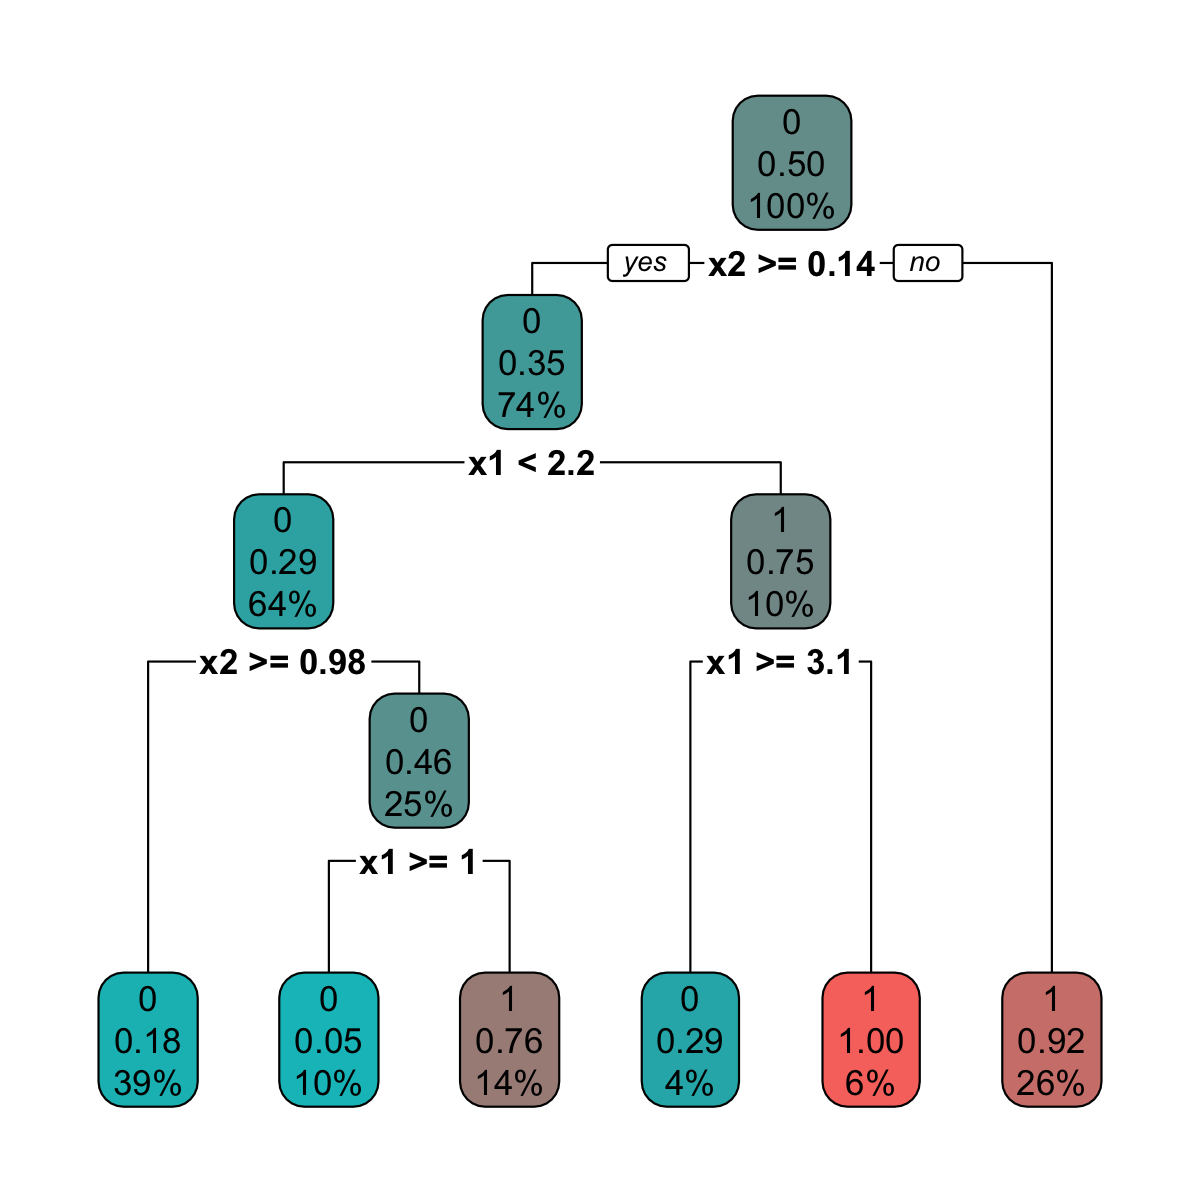
\includegraphics[width=0.6\textwidth]{img/esl-decision-tree-just-tree.png}
\end{center}
And here is the decision boundary produced by this tree:
\begin{center}
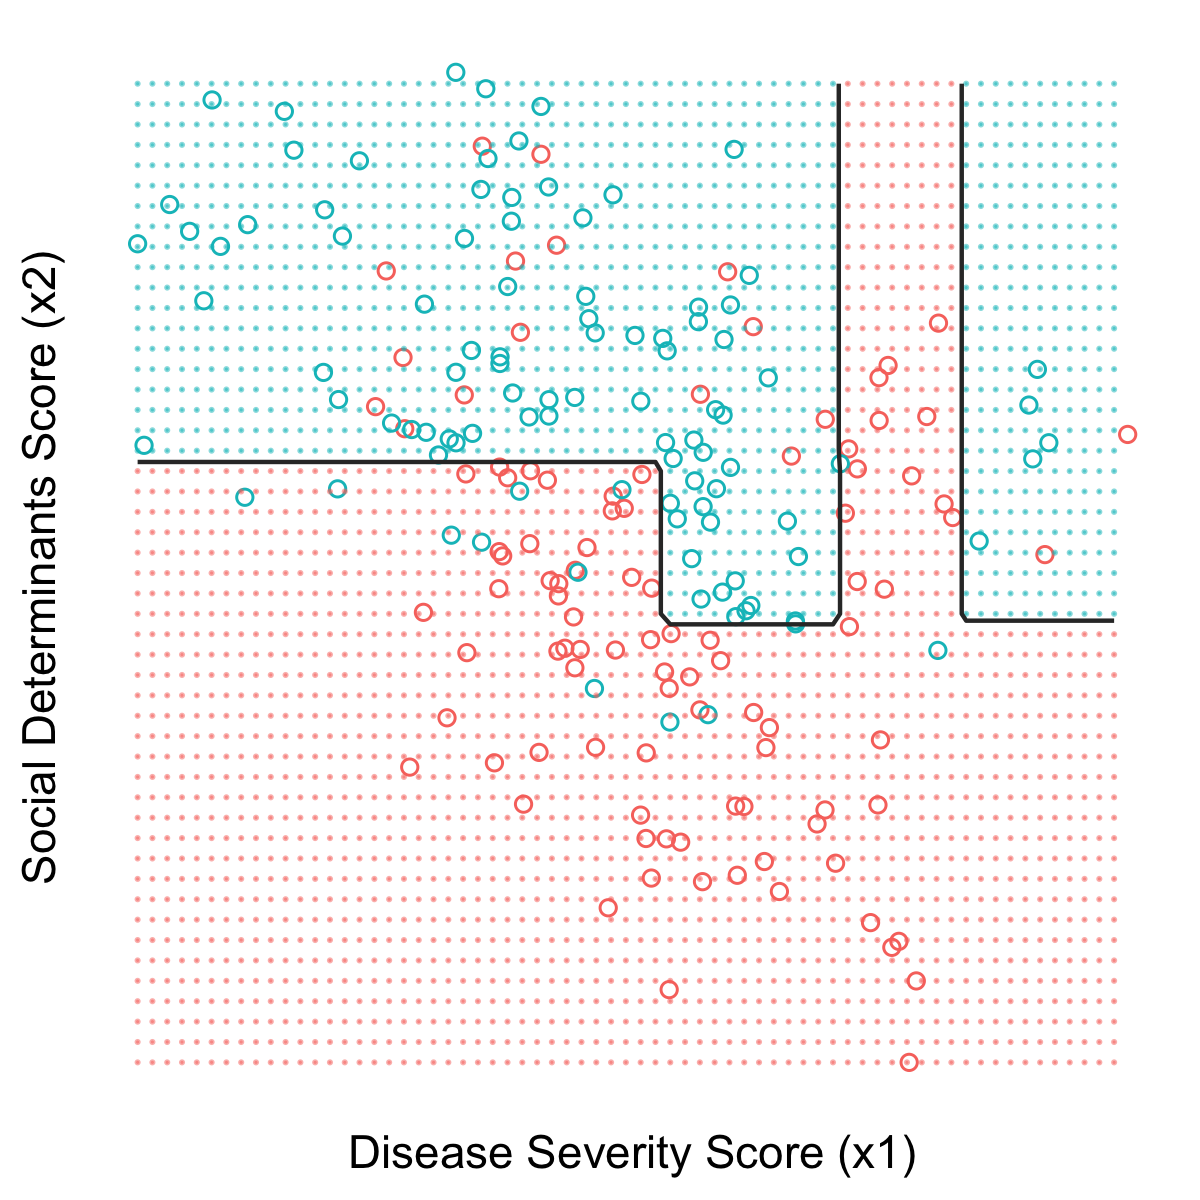
\includegraphics[width=0.7\textwidth]{img/esl-decision-tree.png}
\end{center}

%%%%%%%%%%%%%%%%%%%%%%%%%%%%%%%%%%%%%%%%%%%%%%%%%%%%%%%%%%%%%%%%%%%%%%%%%%%%%%%%%%%%%%

\section{Discussion Questions}

Logistic regression, KNN, and decision trees are three distinct types of classification algorithms. Fed the same training data, they produce three very different-looking decision boundaries.

\begin{enumerate}
\item What are the advantages and disadvantages of the decision boundaries produced by:
  \begin{enumerate}
  \item Logistic regression?
  \item KNN ($K=15$)?
  \item Decision tree?
  \end{enumerate}
\item What are the advantages and disadvantages of KNN with low $K$ (e.g. $K=3$) vs. high $K$ (e.g. $K=50$)? The decision boundaries for the previous example with (left to right) $K=3, 15,$ and $50$ are shown below.
\begin{center}
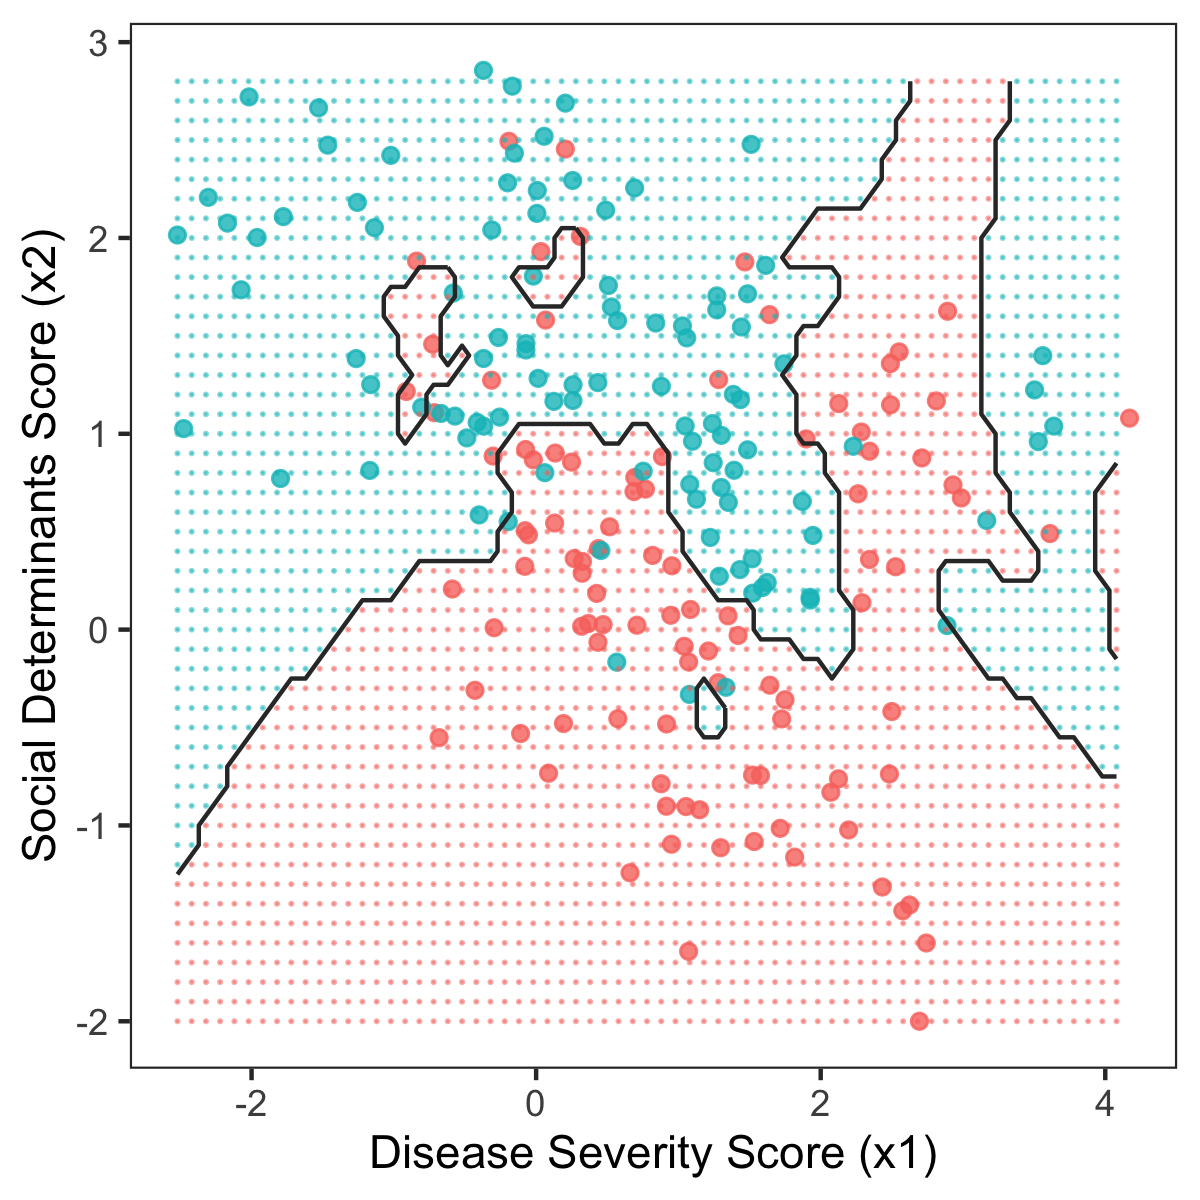
\includegraphics[width=0.3\textwidth]{img/esl-knn-3.png}
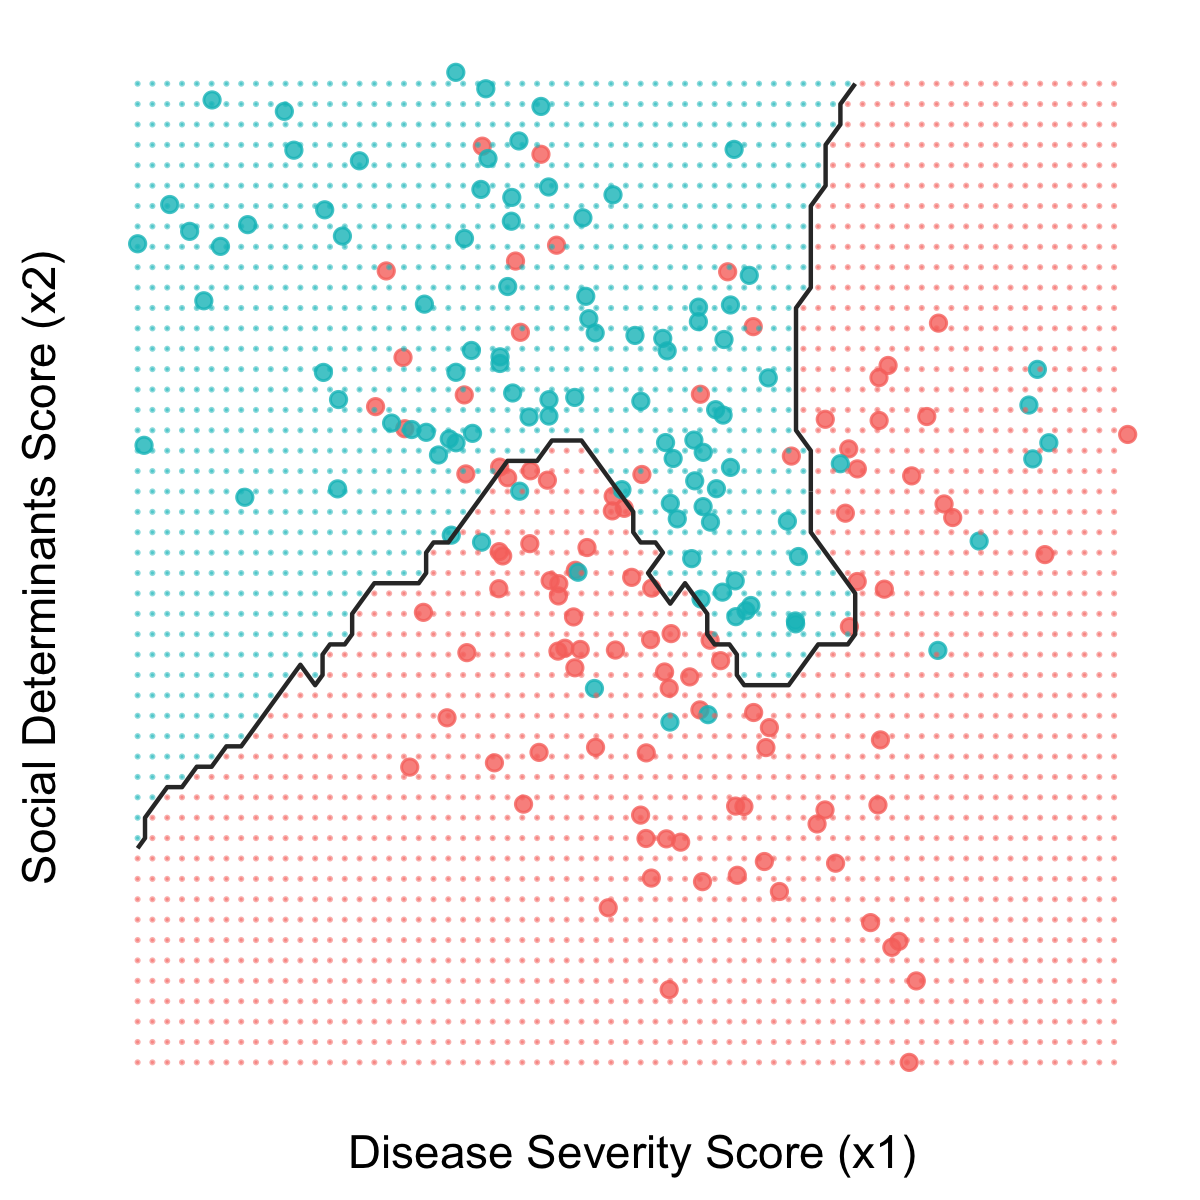
\includegraphics[width=0.3\textwidth]{img/esl-knn-15.png}
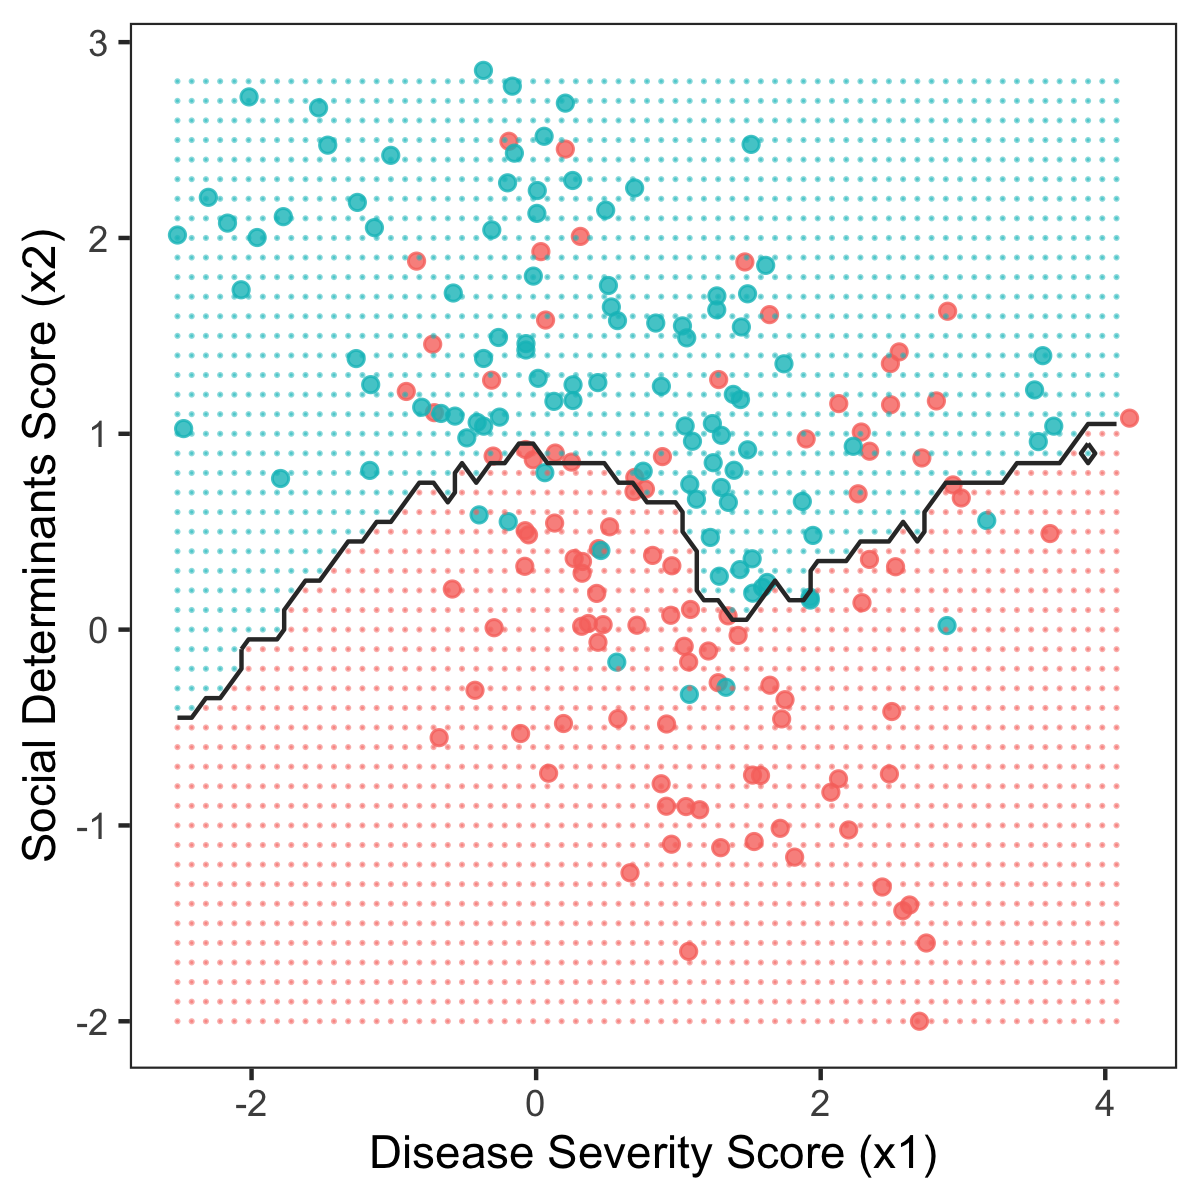
\includegraphics[width=0.3\textwidth]{img/esl-knn-50.png}
\end{center}
\item What makes a good decision boundary?
\item The logistic regression, KNN, and decision tree algorithms can all be applied to address multi-outcome (i.e. more than two categories) classification problems with only minor modifications. Describe how each could be modified to work in these situations. (Think through this yourself before you Google.)
\end{enumerate}



